\section{Git Kraken}
\begin{frame}[allowframebreaks]
\frametitle{Git Kraken}

\begin{itemize}
 \item dostupan za uporabu na Windows, Linux i Mac os operacijskim sustavima


 \item \textbf{Namjena:} 
 \item osnažiti produktivnost Git korisnika kroz \textbf{značajke} kao što su:
  {\setlength\itemindent{15pt}\item vizualna interakcija i savjeti}
  {\setlength\itemindent{15pt}\item samostalnost, učinkovitost, pouzdanost}
  {\setlength\itemindent{15pt}\item podržavanje više profila}
  {\setlength\itemindent{15pt}\item podržavanje funkcije poništavanja i ponovnog odabira jednim klikom}
  {\setlength\itemindent{15pt}\item ugrađeni alat za spajanje}
  {\setlength\itemindent{15pt}\item brz i intuitivan alat za pretraživanje}
  {\setlength\itemindent{15pt}\item prilagodljivost korisničkom radnom prostoru}
  {\setlength\itemindent{15pt}\item podržava i submodule i Gitflow}
  {\setlength\itemindent{15pt}\item integrira se s korisnikovim GitHub ili Bitbucket računom}
  {\setlength\itemindent{15pt}\item tipkovnički prečaci...}
 \framebreak
 \item radi sve standardne stvari koje bi trebali učiniti s git klijentom:
 		\item \textit{grananje}
 		\item \textit{spajanje}
 		\item \textit{povlačenje}
 		\item \textit{guranje}
 		\item \textit{vraćanje}
\framebreak
\item koristan za vizualizaciju prošlih radova

\end{itemize}

\begin{center}
    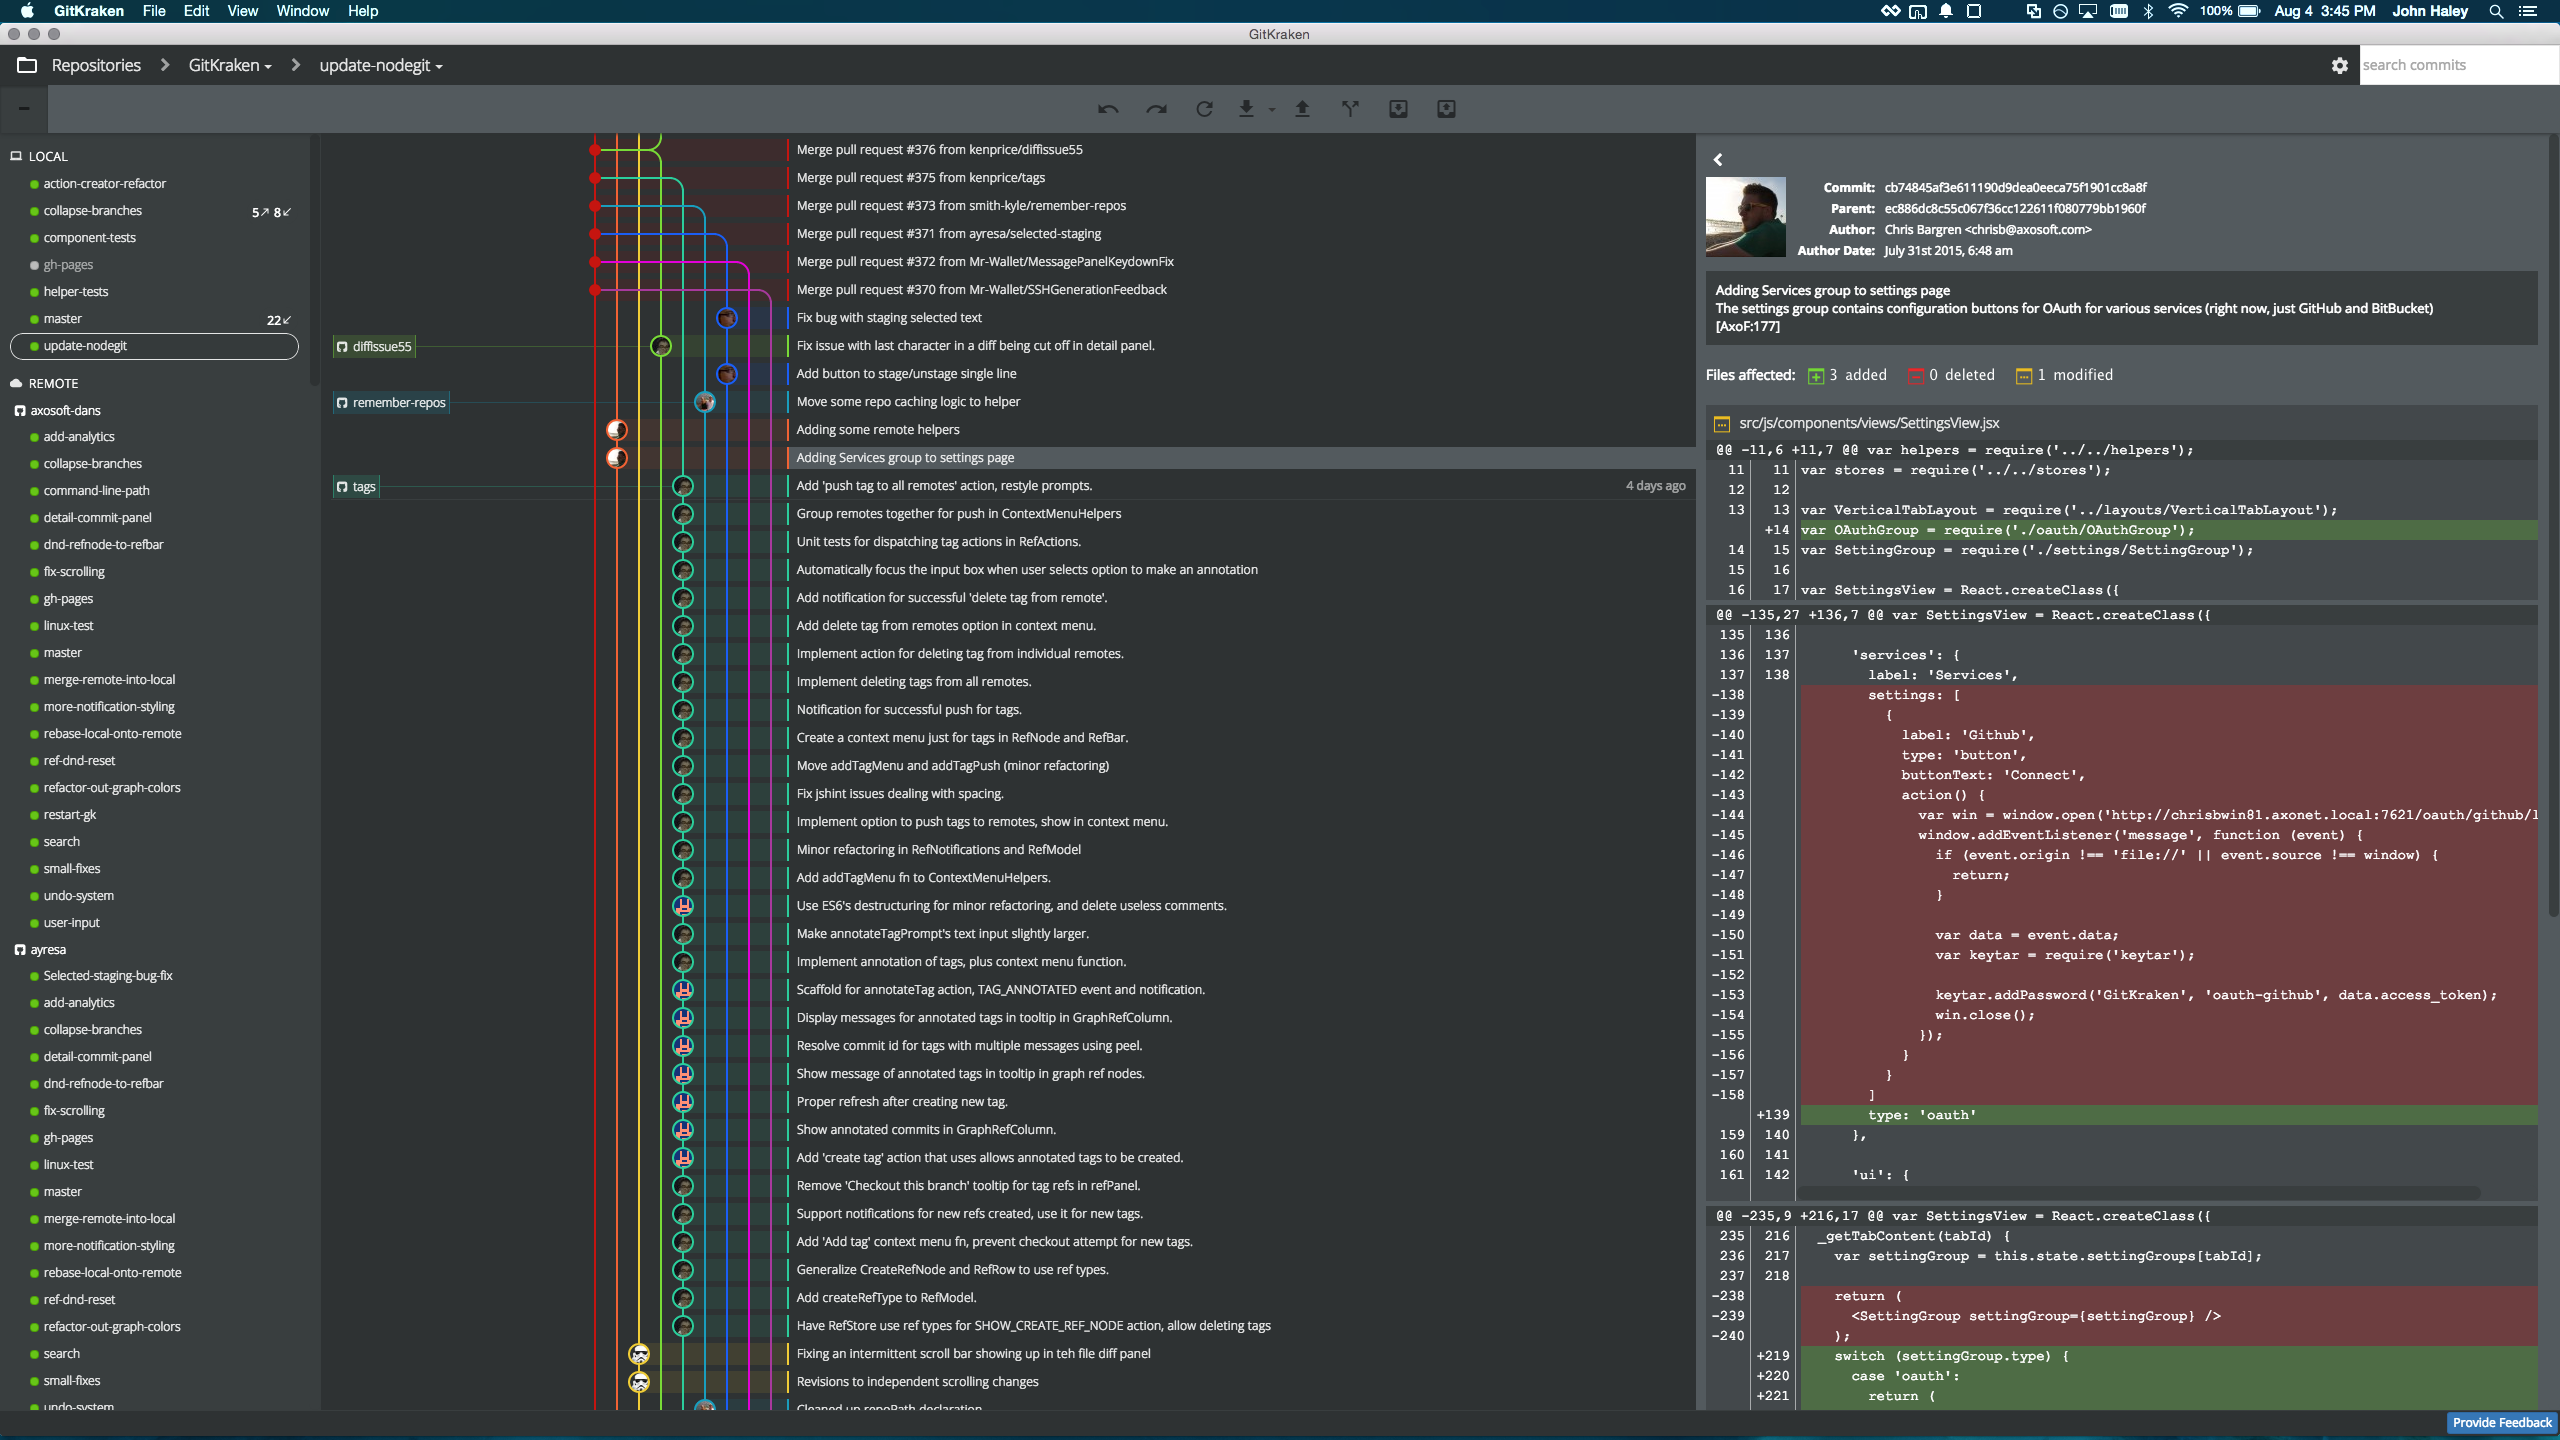
\includegraphics[width=0.8\linewidth]{images/gitkraken-UI.png}
\end{center}

\end{frame}